\documentclass{article}

\usepackage{amsmath}
\usepackage{amssymb}
\usepackage{amsthm}
\usepackage{tikz}
\usepackage{listings}
\usepackage{hyperref}
\usepackage[margin=1in]{geometry}
\usepackage{xcolor}

\usetikzlibrary{arrows.meta,calc,3d}

\lstset{
  language=JavaScript,
  basicstyle=\ttfamily\footnotesize,
  keywordstyle=\color{blue!70!black},
  commentstyle=\color{green!50!black}\itshape,
  stringstyle=\color{red!60!black},
  numbers=left,
  numberstyle=\tiny\color{gray},
  numbersep=6pt,
  showstringspaces=false,
  breaklines=true,
  frame=single,
  framesep=4pt,
  xleftmargin=10pt
}

\title{Guide 01: Vectors and 3D Space}
\author{}
\date{}

\begin{document}
\maketitle

\section{Why this matters}

Almost every nontrivial line of \texttt{web-3d-panel-navigation} is a vector
operation in disguise. The camera transition logic in
\texttt{src/camera-transitions.ts} subtracts two positions to get a forward
direction, normalizes it, dot-products it with another direction, clamps the
result to $[-1,1]$, and feeds it to \texttt{Math.acos}
(\texttt{src/camera-transitions.ts:64--71}). The detail-camera placement in
\texttt{src/camera-controller.ts:62--78} pushes a camera away from a panel
along the panel's normal vector by a scalar distance. The tile-layout code in
\texttt{src/zoom-plane-parser.ts:416--429} builds a panel offset by scaling the
parent panel's local right and up vectors and adding them. The bounding-box
projection in \texttt{src/projection.ts:23--48} treats every plane corner as a
triple $(x, y, z)$ and aggregates componentwise minima and maxima. To read
this codebase you must read it in vectors.

This guide is the foundation. We build 3D vectors from the ground up,
introduce magnitude, addition, scalar multiplication, normalization, and the
dot product, and then show those exact operations in the project's source.

\section{Building intuition}

\subsection{Points versus directions}

A point in 3D space is a location: ``the panel is at $(2, 1, -3)$.'' A
direction is an arrow with no location: ``the camera is looking down the
$+z$ axis.'' Both are stored as ordered triples of numbers, but they behave
differently. Subtracting two points gives a direction (``go from here to
there''). Adding a direction to a point gives a new point. Adding two points
is geometrically meaningless, even though the arithmetic is defined.

\begin{center}
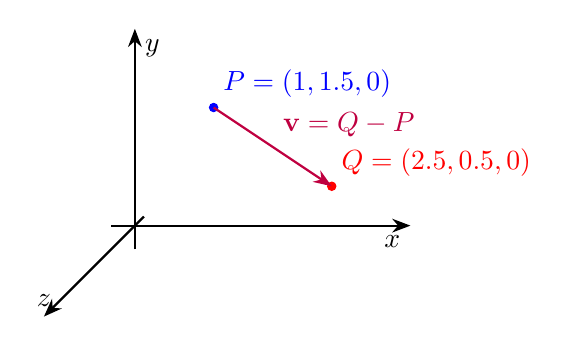
\begin{tikzpicture}[scale=1.0,>=Stealth]
  \draw[->, thick] (-0.3,0,0) -- (3.5,0,0) node[anchor=north east]{$x$};
  \draw[->, thick] (0,-0.3,0) -- (0,2.5,0) node[anchor=north west]{$y$};
  \draw[->, thick] (0,0,-0.3) -- (0,0,3) node[anchor=south]{$z$};

  \filldraw[blue] (1,1.5,0) circle (1.5pt) node[above right] {$P = (1,1.5,0)$};
  \filldraw[red]  (2.5,0.5,0) circle (1.5pt) node[above right] {$Q = (2.5, 0.5, 0)$};
  \draw[->, thick, purple] (1,1.5,0) -- (2.5,0.5,0) node[midway, above right] {$\mathbf{v} = Q - P$};
\end{tikzpicture}
\end{center}

The purple arrow is a direction; the blue and red dots are points. Notice
that $\mathbf{v} = Q - P$ has no inherent location. We \emph{drew} it
starting at $P$, but it is the same arrow if we draw it anywhere.

\subsection{Three operations, three pictures}

\noindent\textbf{Addition (head-to-tail).} To add two vectors, draw the second
starting where the first ends. The sum is the arrow from the first tail to
the last head.

\begin{center}
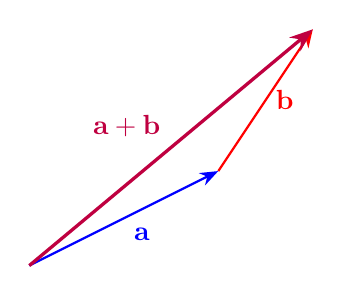
\begin{tikzpicture}[scale=1.2,>=Stealth]
  \draw[->, thick, blue]   (0,0) -- (2,1) node[midway, below right] {$\mathbf{a}$};
  \draw[->, thick, red]    (2,1) -- (3,2.5) node[midway, right] {$\mathbf{b}$};
  \draw[->, very thick, purple] (0,0) -- (3,2.5) node[midway, above left] {$\mathbf{a}+\mathbf{b}$};
\end{tikzpicture}
\end{center}

\noindent\textbf{Scalar multiplication.} Multiplying a vector by a positive
number scales its length. Multiplying by a negative number flips it.

\begin{center}
\begin{tikzpicture}[scale=1.0,>=Stealth]
  \draw[->, thick, blue]   (0,0) -- (1.5,0.5) node[midway, above] {$\mathbf{v}$};
  \draw[->, thick, red]    (3,0) -- (6,1) node[midway, above] {$2\mathbf{v}$};
  \draw[->, thick, green!50!black] (8,0) -- (7.25,-0.25) node[midway, below] {$-0.5\mathbf{v}$};
\end{tikzpicture}
\end{center}

\noindent\textbf{Normalization.} Dividing a vector by its own length yields a
unit vector --- same direction, length 1. This is how the project converts
``the line from camera to target'' into ``which way is the camera looking,''
discarding the distance.

\begin{center}
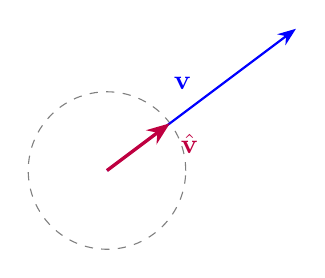
\begin{tikzpicture}[scale=1.0,>=Stealth]
  \draw[dashed, gray] (0,0) circle (1cm);
  \draw[->, thick, blue] (0,0) -- (2.4,1.8) node[midway, above left] {$\mathbf{v}$};
  \draw[->, very thick, purple] (0,0) -- (0.8,0.6) node[below right] {$\hat{\mathbf{v}}$};
\end{tikzpicture}
\end{center}

\section{The math}

\subsection{3D vectors}

A 3D vector is an ordered triple of real numbers
\[
\mathbf{v} = \begin{pmatrix} v_x \\ v_y \\ v_z \end{pmatrix} \in \mathbb{R}^3.
\]
We write $\mathbf{v}$ in bold; its components are $v_x, v_y, v_z$. We use the
same notation for points; whether the triple represents a position or a
direction is a matter of intent, not type. Three.js makes the same choice:
\texttt{THREE.Vector3} stores both.

\subsection{Magnitude}

The magnitude (or length, or norm) of $\mathbf{v}$ is
\[
\|\mathbf{v}\| = \sqrt{v_x^2 + v_y^2 + v_z^2}.
\]
This is the Pythagorean theorem applied twice. In the $xy$-plane, the
diagonal has length $\sqrt{v_x^2 + v_y^2}$; that diagonal and $v_z$ form a
right triangle with hypotenuse $\sqrt{v_x^2 + v_y^2 + v_z^2}$.

\subsection{Addition and subtraction}

Addition and subtraction are componentwise:
\[
\mathbf{a} + \mathbf{b} = \begin{pmatrix} a_x + b_x \\ a_y + b_y \\ a_z + b_z \end{pmatrix},
\qquad
\mathbf{a} - \mathbf{b} = \begin{pmatrix} a_x - b_x \\ a_y - b_y \\ a_z - b_z \end{pmatrix}.
\]
Both are commutative for addition ($\mathbf{a}+\mathbf{b} = \mathbf{b}+\mathbf{a}$)
and associative ($(\mathbf{a}+\mathbf{b})+\mathbf{c} = \mathbf{a}+(\mathbf{b}+\mathbf{c})$).
Subtraction is just addition of the negation.

\subsection{Scalar multiplication}

For $s \in \mathbb{R}$,
\[
s\mathbf{v} = \begin{pmatrix} s v_x \\ s v_y \\ s v_z \end{pmatrix}.
\]
A useful property:
$\|s\mathbf{v}\| = |s| \cdot \|\mathbf{v}\|$. If you scale a vector by $s$, you
scale its length by $|s|$.

\subsection{Normalization}

Given any nonzero $\mathbf{v}$, we can construct the unit vector pointing the
same way:
\[
\hat{\mathbf{v}} = \frac{\mathbf{v}}{\|\mathbf{v}\|}.
\]
We verify $\|\hat{\mathbf{v}}\| = 1$:
\[
\|\hat{\mathbf{v}}\| = \left\|\frac{1}{\|\mathbf{v}\|}\mathbf{v}\right\|
   = \frac{1}{\|\mathbf{v}\|}\|\mathbf{v}\| = 1.
\]
This is a recurring trick in the project: \emph{strip distance, keep
direction.}

\subsection{The dot product, algebraically}

\[
\mathbf{a} \cdot \mathbf{b} = a_x b_x + a_y b_y + a_z b_z.
\]
The dot product takes two vectors and returns a single scalar. Properties:
\begin{itemize}
  \item Commutative: $\mathbf{a} \cdot \mathbf{b} = \mathbf{b} \cdot \mathbf{a}$.
  \item Distributes over addition: $\mathbf{a} \cdot (\mathbf{b}+\mathbf{c}) = \mathbf{a}\cdot\mathbf{b} + \mathbf{a}\cdot\mathbf{c}$.
  \item Self-dot is squared length: $\mathbf{v} \cdot \mathbf{v} = \|\mathbf{v}\|^2$.
\end{itemize}
The last identity falls straight out of the formula:
$\mathbf{v} \cdot \mathbf{v} = v_x^2 + v_y^2 + v_z^2 = \|\mathbf{v}\|^2$.

\subsection{The dot product, geometrically}

The geometric identity is
\[
\mathbf{a} \cdot \mathbf{b} = \|\mathbf{a}\|\,\|\mathbf{b}\|\cos\theta,
\]
where $\theta$ is the angle between $\mathbf{a}$ and $\mathbf{b}$ when their
tails are placed at the same point. Here is a derivation by the law of
cosines.

\begin{proof}[Derivation]
Place $\mathbf{a}$ and $\mathbf{b}$ tail-to-tail. The third side of the
triangle they form is $\mathbf{a}-\mathbf{b}$. The law of cosines says
\[
\|\mathbf{a}-\mathbf{b}\|^2 = \|\mathbf{a}\|^2 + \|\mathbf{b}\|^2 - 2\|\mathbf{a}\|\|\mathbf{b}\|\cos\theta.
\]
Expand the left side using the algebraic identity $\mathbf{v}\cdot\mathbf{v} = \|\mathbf{v}\|^2$ and distributivity:
\begin{align*}
\|\mathbf{a}-\mathbf{b}\|^2
   &= (\mathbf{a}-\mathbf{b})\cdot(\mathbf{a}-\mathbf{b}) \\
   &= \mathbf{a}\cdot\mathbf{a} - 2\,\mathbf{a}\cdot\mathbf{b} + \mathbf{b}\cdot\mathbf{b} \\
   &= \|\mathbf{a}\|^2 - 2\,\mathbf{a}\cdot\mathbf{b} + \|\mathbf{b}\|^2.
\end{align*}
Setting the two expressions for $\|\mathbf{a}-\mathbf{b}\|^2$ equal and
canceling the $\|\mathbf{a}\|^2 + \|\mathbf{b}\|^2$ terms gives
\[
-2\,\mathbf{a}\cdot\mathbf{b} = -2\|\mathbf{a}\|\|\mathbf{b}\|\cos\theta,
\]
so $\mathbf{a}\cdot\mathbf{b} = \|\mathbf{a}\|\|\mathbf{b}\|\cos\theta$.
\end{proof}

\subsection{Dot product as projection}

If $\hat{\mathbf{u}}$ is a unit vector, then
$\mathbf{a} \cdot \hat{\mathbf{u}} = \|\mathbf{a}\| \cos\theta$ is the
\emph{signed length} of the shadow $\mathbf{a}$ casts on the line through
$\hat{\mathbf{u}}$. Positive if $\mathbf{a}$ points roughly the same way as
$\hat{\mathbf{u}}$, negative if opposite, zero if perpendicular.

\begin{center}
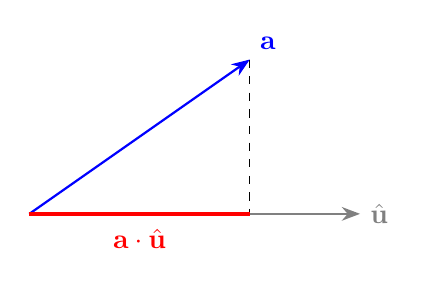
\begin{tikzpicture}[scale=1.4,>=Stealth]
  \draw[->, thick, gray] (0,0) -- (3,0) node[right] {$\hat{\mathbf{u}}$};
  \draw[->, thick, blue] (0,0) -- (2,1.4) node[above right] {$\mathbf{a}$};
  \draw[dashed] (2,1.4) -- (2,0);
  \draw[very thick, red] (0,0) -- (2,0);
  \node[below, red] at (1,-0.05) {$\mathbf{a}\cdot\hat{\mathbf{u}}$};
\end{tikzpicture}
\end{center}

\subsection{Unit vectors and the cosine identity}

If both $\hat{\mathbf{u}}$ and $\hat{\mathbf{v}}$ are unit vectors, the
geometric formula collapses to
\[
\hat{\mathbf{u}} \cdot \hat{\mathbf{v}} = \cos\theta.
\]
This is the workhorse identity of the codebase. Whenever you see two
\texttt{normalize()} calls followed by a \texttt{.dot()}, the program is
asking ``what is the cosine of the angle between these two directions?''.

\subsection{Numerical safety: clamp before \texttt{acos}}

Floating-point arithmetic does not respect the inequality $|\hat{\mathbf{u}} \cdot \hat{\mathbf{v}}| \le 1$
exactly. Two unit vectors that should give a dot of $1$ can give $1.0000000002$.
Feeding that to \texttt{Math.acos} returns \texttt{NaN}. The fix is to clamp
the dot product to $[-1, 1]$ first:
\begin{lstlisting}
const dot = THREE.MathUtils.clamp(fromDir.dot(toDir), -1, 1);
const theta = Math.acos(dot);
\end{lstlisting}
We will derive \texttt{acos} itself in guide 02. For now: clamp first, ask
later.

\section{In this codebase}

\subsection{Subtract, normalize, dot, clamp --- the angle pipeline}

\texttt{src/camera-transitions.ts:63--71} packs four ideas from this guide
into a five-line block: subtract two points to get a direction, normalize
it, dot two directions, and clamp before \texttt{acos}.

\begin{lstlisting}
// Forward angle
const fromFwd = new THREE.Vector3().subVectors(from.target, from.position).normalize();
const toFwd = new THREE.Vector3().subVectors(to.target, to.position).normalize();
const fwdDot = THREE.MathUtils.clamp(fromFwd.dot(toFwd), -1, 1);
const fwdAngle = Math.acos(fwdDot);

// Up angle (captures roll/tilt that forward angle misses)
const upDot = THREE.MathUtils.clamp(from.up.dot(to.up), -1, 1);
const upAngle = Math.acos(upDot);
\end{lstlisting}

Mathematically, line by line:
\begin{itemize}
  \item \texttt{subVectors(target, position)} computes $\mathbf{t} - \mathbf{p}$, the direction from camera to its target.
  \item \texttt{.normalize()} divides by length. After this call, both \texttt{fromFwd} and \texttt{toFwd} are unit vectors.
  \item \texttt{fromFwd.dot(toFwd)} is $\hat{\mathbf{f}}_{\text{from}} \cdot \hat{\mathbf{f}}_{\text{to}} = \cos\theta_{\text{fwd}}$.
  \item The clamp guards against floating-point overshoot. The \texttt{acos} is what guide 02 will explain.
\end{itemize}
The same pipeline runs again for \texttt{from.up} and \texttt{to.up}, which
are already unit vectors so no \texttt{.normalize()} is needed.

\subsection{Push the camera along a normal --- scalar multiplication and addition}

\texttt{src/camera-controller.ts:59--78} computes where to put the camera so
that it views a panel head-on at distance $d$. The pattern is
\emph{point + scalar $\cdot$ direction}.

\begin{lstlisting}
const euler = new THREE.Euler(plane.rotation[0], plane.rotation[1], plane.rotation[2]);

// Plane's normal vector (perpendicular, pointing toward viewer)
const normal = new THREE.Vector3(0, 0, 1);
normal.applyEuler(euler);
normal.normalize();

// Plane's local "up" vector - aligns with screen vertical when viewing head-on
const planeUp = new THREE.Vector3(0, 1, 0);
planeUp.applyEuler(euler);
planeUp.normalize();

const planeCenter = new THREE.Vector3(
  plane.position[0],
  plane.position[1],
  plane.position[2]
);

// Camera position: plane center + (normal * distance)
const cameraPosition = planeCenter.clone().add(normal.clone().multiplyScalar(distance));
\end{lstlisting}

The last line is the formula
\[
\mathbf{p}_{\text{camera}} = \mathbf{p}_{\text{plane}} + d \, \hat{\mathbf{n}}.
\]
We start from the panel's center (a point), scale the unit normal by the
scalar \texttt{distance} (a direction with chosen length), and add. The
\texttt{.clone()} calls exist because Three.js's \texttt{add} and
\texttt{multiplyScalar} mutate the receiver; cloning keeps the originals
untouched. We will defer the rotation step (\texttt{applyEuler}) until guide
04 --- for now, treat \texttt{normal} as a unit vector that has been pointed
in some direction.

\subsection{Local-space offsets via two scaled basis vectors}

\texttt{src/zoom-plane-parser.ts:416--429} builds a tile offset by combining
the parent panel's local right and up axes. This is the same ``point plus
scaled direction'' pattern, but with two directions added.

\begin{lstlisting}
const referenceCenter = new THREE.Vector3(
  reference.position[0],
  reference.position[1],
  reference.position[2]
);
const referenceQuaternion = new THREE.Quaternion().setFromEuler(
  new THREE.Euler(reference.rotation[0], reference.rotation[1], reference.rotation[2], 'XYZ')
);
const referenceRight = new THREE.Vector3(1, 0, 0).applyQuaternion(referenceQuaternion);
const referenceUp = new THREE.Vector3(0, 1, 0).applyQuaternion(referenceQuaternion);
const finalOffset = calculateErgonomicTileOffset(layout, definition, reference, scale);
const hingeOffset = referenceRight.clone()
  .multiplyScalar(finalOffset[0])
  .add(referenceUp.clone().multiplyScalar(finalOffset[1]));
\end{lstlisting}

The last expression is
\[
\mathbf{o} = (\text{offset}_x)\,\hat{\mathbf{r}} + (\text{offset}_y)\,\hat{\mathbf{u}}.
\]
Two unit vectors, each scaled by a scalar, then added. This produces a
displacement vector $\mathbf{o}$ that lives in the panel's local plane. To
get a world point, you would add this displacement to a world point such as
\texttt{referenceCenter}, which is exactly what the surrounding code does.

\subsection{Componentwise aggregation --- vectors are triples}

\texttt{src/projection.ts:23--48} reminds us that a vector is ultimately
three numbers. The bounding-box loop walks every plane corner and tracks the
min and max along each axis independently.

\begin{lstlisting}
let minX = Infinity, maxX = -Infinity;
let minY = Infinity, maxY = -Infinity;
let minZ = Infinity, maxZ = -Infinity;

for (const config of configs) {
  const corners = getPlaneWorldCorners(config, scale);
  for (const corner of corners) {
    minX = Math.min(minX, corner.x);
    maxX = Math.max(maxX, corner.x);
    minY = Math.min(minY, corner.y);
    maxY = Math.max(maxY, corner.y);
    minZ = Math.min(minZ, corner.z);
    maxZ = Math.max(maxZ, corner.z);
  }
}
\end{lstlisting}

There is no fancy vector identity here. The point is the opposite: the $x$,
$y$, and $z$ axes are independent slots, and any operation that does not
mix them (addition, subtraction, scalar multiplication, componentwise min /
max) decomposes into three scalar operations. Every vector identity in this
guide is, at the bytes-on-the-CPU level, three scalar identities running in
parallel.

\section{Worked examples}

\subsection*{Example 1: Length of a forward vector}

A camera sits at $\mathbf{p} = (0, 2, 5)$ and looks at the panel center
$\mathbf{t} = (0, 0, 0)$. What unit forward vector does the
\texttt{subVectors / normalize} pipeline produce?

\textbf{Step 1: Subtract.} The forward direction (unnormalized) is
\[
\mathbf{f} = \mathbf{t} - \mathbf{p} = (0-0,\ 0-2,\ 0-5) = (0, -2, -5).
\]

\textbf{Step 2: Length.}
\[
\|\mathbf{f}\| = \sqrt{0^2 + (-2)^2 + (-5)^2} = \sqrt{29} \approx 5.385.
\]

\textbf{Step 3: Normalize.}
\[
\hat{\mathbf{f}} = \frac{1}{\sqrt{29}}(0, -2, -5)
   \approx (0,\ -0.371,\ -0.928).
\]
Sanity check: $0^2 + 0.371^2 + 0.928^2 \approx 0.999 \approx 1$. The small
error is exactly why the project clamps before \texttt{acos}.

\subsection*{Example 2: Camera placement along a normal}

Suppose \texttt{calculatePerpendicularState} has determined the panel center
is $\mathbf{c} = (1, 0, 0)$, the panel normal is $\hat{\mathbf{n}} = (0, 0, 1)$
(panel facing $+z$), and the required distance is $d = 4$. Where does the
camera go?

\[
\mathbf{p}_{\text{camera}} = \mathbf{c} + d\,\hat{\mathbf{n}}
   = (1, 0, 0) + 4\cdot(0, 0, 1) = (1, 0, 4).
\]
Notice that $\hat{\mathbf{n}}$ being a unit vector is what makes
\texttt{distance} interpretable as ``how far in world units.'' If
$\hat{\mathbf{n}}$ were unnormalized of length $2$, the same code would put
the camera at distance $8$, not $4$. This is why the source calls
\texttt{normal.normalize()} before \texttt{multiplyScalar(distance)}.

\subsection*{Example 3: Cosine of the angle between two camera-forwards}

The first camera looks straight down $-z$: $\hat{\mathbf{f}}_1 = (0, 0, -1)$.
The second has been rotated and looks down a diagonal:
$\hat{\mathbf{f}}_2 = (0, -\tfrac{1}{\sqrt{2}}, -\tfrac{1}{\sqrt{2}})$. What
does \texttt{fromFwd.dot(toFwd)} return, and what is the angle?

\textbf{Dot product.}
\[
\hat{\mathbf{f}}_1 \cdot \hat{\mathbf{f}}_2
   = (0)(0) + (0)\!\left(-\tfrac{1}{\sqrt{2}}\right) + (-1)\!\left(-\tfrac{1}{\sqrt{2}}\right)
   = \frac{1}{\sqrt{2}} \approx 0.7071.
\]

\textbf{Angle.} Since both vectors are unit, $\cos\theta = \tfrac{1}{\sqrt{2}}$,
so $\theta = 45^\circ$. This would feed into \texttt{fwdAngle} in
\texttt{camera-transitions.ts} and contribute to the regime decision (early
look vs.\ orbit) at the $30^\circ$/$35^\circ$ thresholds.

\section{Exercises}

\begin{enumerate}
  \item Compute $\|\mathbf{v}\|$ for $\mathbf{v} = (3, 4, 12)$, and write down $\hat{\mathbf{v}}$.

  \item Two camera positions are $\mathbf{p}_a = (5, 0, 0)$ and $\mathbf{p}_b = (1, 0, 3)$, both looking at the origin. Compute their forward unit vectors and the dot product between them.

  \item Two unit vectors satisfy $\hat{\mathbf{u}} \cdot \hat{\mathbf{v}} = 0$. What is the angle between them? Sketch an example pair in 2D.

  \item Suppose a panel has center $\mathbf{c} = (2, 1, -3)$ and unit normal $\hat{\mathbf{n}} = \left(\tfrac{1}{\sqrt{2}}, 0, \tfrac{1}{\sqrt{2}}\right)$. Where should the camera sit if \texttt{distance} is $\sqrt{2}$?

  \item Explain in one or two sentences why \texttt{src/camera-transitions.ts} clamps the dot product to $[-1, 1]$ before passing it to \texttt{Math.acos}, even though mathematically the dot of two unit vectors should already lie in $[-1, 1]$.

  \item (Conceptual.) The bounding-box loop in \texttt{src/projection.ts} treats the $x$, $y$, and $z$ axes independently. Could it use a single ``vector min'' that mixes axes (for example, the corner with smallest \emph{magnitude})? Why or why not, in terms of what a bounding box is supposed to represent?

  \item (Project-applied.) In \texttt{calculatePerpendicularState}, the line \texttt{normal.normalize()} appears immediately before the camera position is computed. Suppose someone deletes that line. The vector \texttt{(0, 0, 1)} fed in is already unit, but after \texttt{applyEuler} (a rotation) it might not be exactly unit due to floating-point drift. Predict, in one sentence, what would happen to camera placement after many rotations if the \texttt{.normalize()} call were removed.
\end{enumerate}

\subsection*{Extension challenges}

\begin{enumerate}
  \setcounter{enumi}{7}
  \item Show algebraically that for any $\mathbf{a}, \mathbf{b} \in \mathbb{R}^3$,
        \[
        \|\mathbf{a}+\mathbf{b}\|^2 + \|\mathbf{a}-\mathbf{b}\|^2 = 2\|\mathbf{a}\|^2 + 2\|\mathbf{b}\|^2.
        \]
        (This is the parallelogram law. Hint: expand each side using $\mathbf{v}\cdot\mathbf{v} = \|\mathbf{v}\|^2$ and distributivity.)

  \item In \texttt{src/zoom-plane-parser.ts:416--429}, the offset
        $\mathbf{o} = \text{offset}_x\,\hat{\mathbf{r}} + \text{offset}_y\,\hat{\mathbf{u}}$ uses two unit vectors. If the panel were rotated $90^\circ$ around the world $y$-axis, its right vector would change but its up vector would not. Predict (without computing the full rotation) which component of the world-space offset $\mathbf{o}$ would be most affected, and explain why $\hat{\mathbf{r}}$ and $\hat{\mathbf{u}}$ being unit vectors is essential for the values of $\text{offset}_x$ and $\text{offset}_y$ to mean ``world units in those directions.''
\end{enumerate}

\section{Where to next}

Guide 02 picks up where this one stops. We have a clamped dot product
sitting in front of \texttt{Math.acos}, but we have not said what
\texttt{acos} actually computes, why $30^\circ$ and $35^\circ$ become
\texttt{30 * THREE.MathUtils.DEG2RAD}, or where \texttt{Math.tan(fovRadians / 2)}
in \texttt{calculatePerpendicularState} comes from. Guide 02 derives the
trigonometric functions, the radian--degree conversion, and the
\texttt{tan(fov/2)} setup that turns a field-of-view angle into a viewing
distance.

\appendix
\section*{Appendix: Solutions}
\addcontentsline{toc}{section}{Appendix: Solutions}

\paragraph{Exercise 1.}
$\|\mathbf{v}\| = \sqrt{9 + 16 + 144} = \sqrt{169} = 13$.
Therefore $\hat{\mathbf{v}} = \tfrac{1}{13}(3, 4, 12) = \left(\tfrac{3}{13}, \tfrac{4}{13}, \tfrac{12}{13}\right)$.

\paragraph{Exercise 2.}
The unnormalized forwards are $\mathbf{f}_a = (0,0,0) - (5,0,0) = (-5, 0, 0)$
with $\|\mathbf{f}_a\| = 5$, so $\hat{\mathbf{f}}_a = (-1, 0, 0)$. Similarly
$\mathbf{f}_b = (-1, 0, -3)$ with $\|\mathbf{f}_b\| = \sqrt{1 + 9} = \sqrt{10}$,
so $\hat{\mathbf{f}}_b = \tfrac{1}{\sqrt{10}}(-1, 0, -3)$. The dot product is
\[
\hat{\mathbf{f}}_a \cdot \hat{\mathbf{f}}_b
  = (-1)\!\left(-\tfrac{1}{\sqrt{10}}\right) + 0 + 0
  = \tfrac{1}{\sqrt{10}} \approx 0.316.
\]

\paragraph{Exercise 3.}
Since both are unit vectors, $\hat{\mathbf{u}} \cdot \hat{\mathbf{v}} = \cos\theta = 0$,
so $\theta = 90^\circ$ (perpendicular). In 2D, an example pair is
$(1, 0)$ and $(0, 1)$.

\paragraph{Exercise 4.}
\[
\mathbf{p}_{\text{camera}} = \mathbf{c} + d\,\hat{\mathbf{n}}
  = (2,1,-3) + \sqrt{2}\cdot\left(\tfrac{1}{\sqrt{2}}, 0, \tfrac{1}{\sqrt{2}}\right)
  = (2+1,\ 1,\ -3+1) = (3, 1, -2).
\]

\paragraph{Exercise 5.}
Floating-point arithmetic can cause the computed dot of two unit vectors to
exceed $1$ (or fall below $-1$) by a tiny amount. \texttt{Math.acos} returns
\texttt{NaN} for any input strictly outside $[-1, 1]$, which would corrupt
the angle computation and the entire transition-blend decision. Clamping
projects the value back into the legal domain.

\paragraph{Exercise 6.}
A bounding box is meant to describe an axis-aligned region: ``what is the
range of $x$ values, the range of $y$ values, the range of $z$ values
across all corners?'' These ranges are computed independently per axis. A
single ``vector min'' that mixes axes (for instance, picking the corner of
smallest magnitude) would discard which corner is extreme along which axis
and would not bound the set of corners at all --- two corners can both have
large magnitude while their $x$ extents are tiny, and the box around them
must still capture both of those $x$ values.

\paragraph{Exercise 7.}
Without renormalization, repeated rotations would let \texttt{normal} drift
slightly in length. Then \texttt{multiplyScalar(distance)} would scale that
incorrect length, so the camera would end up at a slightly wrong distance
from the panel --- closer or farther than \texttt{distance} requested ---
and the error could compound across many transitions, eventually
producing a visibly wrong framing.

\paragraph{Extension 8.}
Expand both squared norms:
\begin{align*}
\|\mathbf{a}+\mathbf{b}\|^2 &= (\mathbf{a}+\mathbf{b})\cdot(\mathbf{a}+\mathbf{b})
  = \|\mathbf{a}\|^2 + 2\,\mathbf{a}\cdot\mathbf{b} + \|\mathbf{b}\|^2, \\
\|\mathbf{a}-\mathbf{b}\|^2 &= (\mathbf{a}-\mathbf{b})\cdot(\mathbf{a}-\mathbf{b})
  = \|\mathbf{a}\|^2 - 2\,\mathbf{a}\cdot\mathbf{b} + \|\mathbf{b}\|^2.
\end{align*}
Adding cancels the $\pm 2\,\mathbf{a}\cdot\mathbf{b}$ terms and leaves
$2\|\mathbf{a}\|^2 + 2\|\mathbf{b}\|^2$, as claimed.

\paragraph{Extension 9.}
Rotating $90^\circ$ around the world $y$-axis sends a panel-local
$\hat{\mathbf{r}} = (1,0,0)$ direction to roughly $(0, 0, \pm 1)$ in world
space, while $\hat{\mathbf{u}} = (0,1,0)$ stays put. So the
$\text{offset}_x \cdot \hat{\mathbf{r}}$ term would now contribute to the
world $z$ component instead of $x$. The $\hat{\mathbf{u}}$ contribution
remains in the world $y$ component. The fact that $\hat{\mathbf{r}}$ and
$\hat{\mathbf{u}}$ are unit vectors is what lets us interpret
$\text{offset}_x$ and $\text{offset}_y$ as honest distances in world units:
$\|s\hat{\mathbf{r}}\| = |s|$ exactly when $\|\hat{\mathbf{r}}\| = 1$.

\end{document}
